% !Rnw weave = knitr
\documentclass[a4paper, french, 11 pt]{article}\usepackage[]{graphicx}\usepackage[]{xcolor}
% maxwidth is the original width if it is less than linewidth
% otherwise use linewidth (to make sure the graphics do not exceed the margin)
\makeatletter
\def\maxwidth{ %
  \ifdim\Gin@nat@width>\linewidth
    \linewidth
  \else
    \Gin@nat@width
  \fi
}
\makeatother

\definecolor{fgcolor}{rgb}{0.345, 0.345, 0.345}
\newcommand{\hlnum}[1]{\textcolor[rgb]{0.686,0.059,0.569}{#1}}%
\newcommand{\hlstr}[1]{\textcolor[rgb]{0.192,0.494,0.8}{#1}}%
\newcommand{\hlcom}[1]{\textcolor[rgb]{0.678,0.584,0.686}{\textit{#1}}}%
\newcommand{\hlopt}[1]{\textcolor[rgb]{0,0,0}{#1}}%
\newcommand{\hlstd}[1]{\textcolor[rgb]{0.345,0.345,0.345}{#1}}%
\newcommand{\hlkwa}[1]{\textcolor[rgb]{0.161,0.373,0.58}{\textbf{#1}}}%
\newcommand{\hlkwb}[1]{\textcolor[rgb]{0.69,0.353,0.396}{#1}}%
\newcommand{\hlkwc}[1]{\textcolor[rgb]{0.333,0.667,0.333}{#1}}%
\newcommand{\hlkwd}[1]{\textcolor[rgb]{0.737,0.353,0.396}{\textbf{#1}}}%
\let\hlipl\hlkwb

\usepackage{framed}
\makeatletter
\newenvironment{kframe}{%
 \def\at@end@of@kframe{}%
 \ifinner\ifhmode%
  \def\at@end@of@kframe{\end{minipage}}%
  \begin{minipage}{\columnwidth}%
 \fi\fi%
 \def\FrameCommand##1{\hskip\@totalleftmargin \hskip-\fboxsep
 \colorbox{shadecolor}{##1}\hskip-\fboxsep
     % There is no \\@totalrightmargin, so:
     \hskip-\linewidth \hskip-\@totalleftmargin \hskip\columnwidth}%
 \MakeFramed {\advance\hsize-\width
   \@totalleftmargin\z@ \linewidth\hsize
   \@setminipage}}%
 {\par\unskip\endMakeFramed%
 \at@end@of@kframe}
\makeatother

\definecolor{shadecolor}{rgb}{.97, .97, .97}
\definecolor{messagecolor}{rgb}{0, 0, 0}
\definecolor{warningcolor}{rgb}{1, 0, 1}
\definecolor{errorcolor}{rgb}{1, 0, 0}
\newenvironment{knitrout}{}{} % an empty environment to be redefined in TeX

\usepackage{alltt}
\usepackage[T1]{fontenc}
\usepackage[utf8]{inputenc}
\usepackage{lmodern}
\usepackage{textcomp}
\usepackage[french]{babel}
\usepackage{graphicx}
\usepackage{geometry}
\geometry{top=2cm, bottom=2cm}
\usepackage{hyperref}
\hypersetup{pdfborder=0 0 0}
\usepackage{epstopdf}
\usepackage{booktabs}
\usepackage[skip=0.5\baselineskip]{caption}
\usepackage[backend=biber, isbn=false, doi=false, url=false, eprint=false, citestyle=ext-authoryear, maxnames=5, hyperref=true]{biblatex}
\DeclareOuterCiteDelims{parencite}{\bibopenbracket}{\bibclosebracket}
\usepackage[french=quotes, csdisplay=true]{csquotes}

\epstopdfDeclareGraphicsRule{.gif}{png}{.png}{convert gif:#1 png:\OutputFile}
\AppendGraphicsExtensions{.gif}
\usepackage{listings}
\usepackage{inconsolata}

\addbibresource{Econometrie.bib}

\title{Les déterminants du salaire au Pays-Bas\\
\vspace{0,5cm}
{\normalsize Projet d'économétrie --- Département de Sciences Humaines et Sociales\\
\vspace{0,5cm}
École normale supérieure Paris-Saclay}}
\author{\normalsize Louis Bourges, Jean-Baptiste Lagrange-Dupuis et Luc Letonturier}
\date{\normalsize\today}
\IfFileExists{upquote.sty}{\usepackage{upquote}}{}
\begin{document}

\maketitle

\section*{Introduction}

Depuis Becker et sa théorie du capital humain en 1964, les travaux économiques visant à expliquer les différences de revenu entre les individus se sont multipliées. Becker a théorisé l’existence d’un calcul coût-avantage microéconomique, qui conduit les individus à arbitrer entre le coût d’une année supplémentaire d’études et le gain espéré à long terme \parencite{becker1964}. Mincer, une décennie plus tard, a enrichi cette approche en incluant l’expérience accumulée au cours des années de travail dans le capital humain \parencite{mincer1974}.

Dans notre étude, nous tenterons de mesurer les effets de ces variables mais aussi d’autres paramètres, à l’instar du genre, de la présence d’enfants, mais aussi des heures travaillées ou de l’âge. Nous nous baserons sur deux enquêtes du LISS\footnote{\textit{Longitudinal Internet studies for the Social Sciences}, les questionnaires sont administrées par Centerdata} menées aux Pays-Bas respectivement en mai 2022 et en septembre 2022. Il s’agira, après une régression classique permettant de comprendre l’influence des différentes variables, de tester la présence d’hétéroscédasticité dans le modèle et, le cas échéant, de la corriger ; de mener un test de Chow pour tenter d'identifier d'éventuels effets de “paliers” quant au lien entre salaire et éducation ainsi que de discuter de la présence d’endogénéité dans le modèle et des moyens à notre disposition pour la corriger. Nous replacerons notre travail dans le contexte de la littérature existante et discuterons aussi de ses limites.



\section{Présentation du modèle et de ses limites}

\subsection{Présentation des variables utilisées}

Nous avons sélectionné plusieurs variables au sein de l’enquête \textit{Work and Schooling} et de la base \textit{Background variables}. La variable \verb+education+, issue d’un recoupement de plusieurs variables, correspond au nombre d’années de scolarité et d’études achevée (c’est-à-dire ayant conduit à l’obtention d’un diplôme), ses valeurs sont comprises entre 0 (personne n’étant jamais allée à l’école) à 22.5 (personne titulaire d’un doctorat, sachant que la scolarité débute à l’âge de 4 ans aux Pays-Bas). La variable \verb+genre+ sépare la population en deux groupes : hommes et femmes, les autres identités de genre ayant été écartées et \verb+age+ indique l’âge des enquêtés. La variable \verb+revenu+ prend en compte le revenu brut mensuel autodéclaré, que nous avons préféré au revenu net, plus dépendant des politiques fiscales et de redistribution. La variable \verb+heures+ correspond au nombre d’heures de travail effectuées en moyenne chaque semaine tandis qu’\verb+experience+ mesure l’ancienneté des salariés dans leur entreprise (en années). Enfin, \verb+nbenfants+ indique le nombre d’enfants présents dans le foyer. 

\subsection{Détection et correction de l’hétéroscédasticité}




Afin de vérifier la présence ou non d’hétéroscédasticité au sein de notre modèle, nous avons réalisé les deux variantes du test de Breusch-Pagan (avec un test de Fisher et avec un test du rapport de vraisemblance) ansi qu’un test de White. Tous concordent et corroborent la présence d’hétéroscédasticité, qui est par ailleurs observable graphiquement : la répartition des résidus en fonction des données prédites n’est pas homogène et l’on observe une forte variabilité de ces résidus en fonction de certaines variables du modèle, notamment la variable heures (Figure \ref{fig:hetero}). 

\begin{figure}[h]
\center
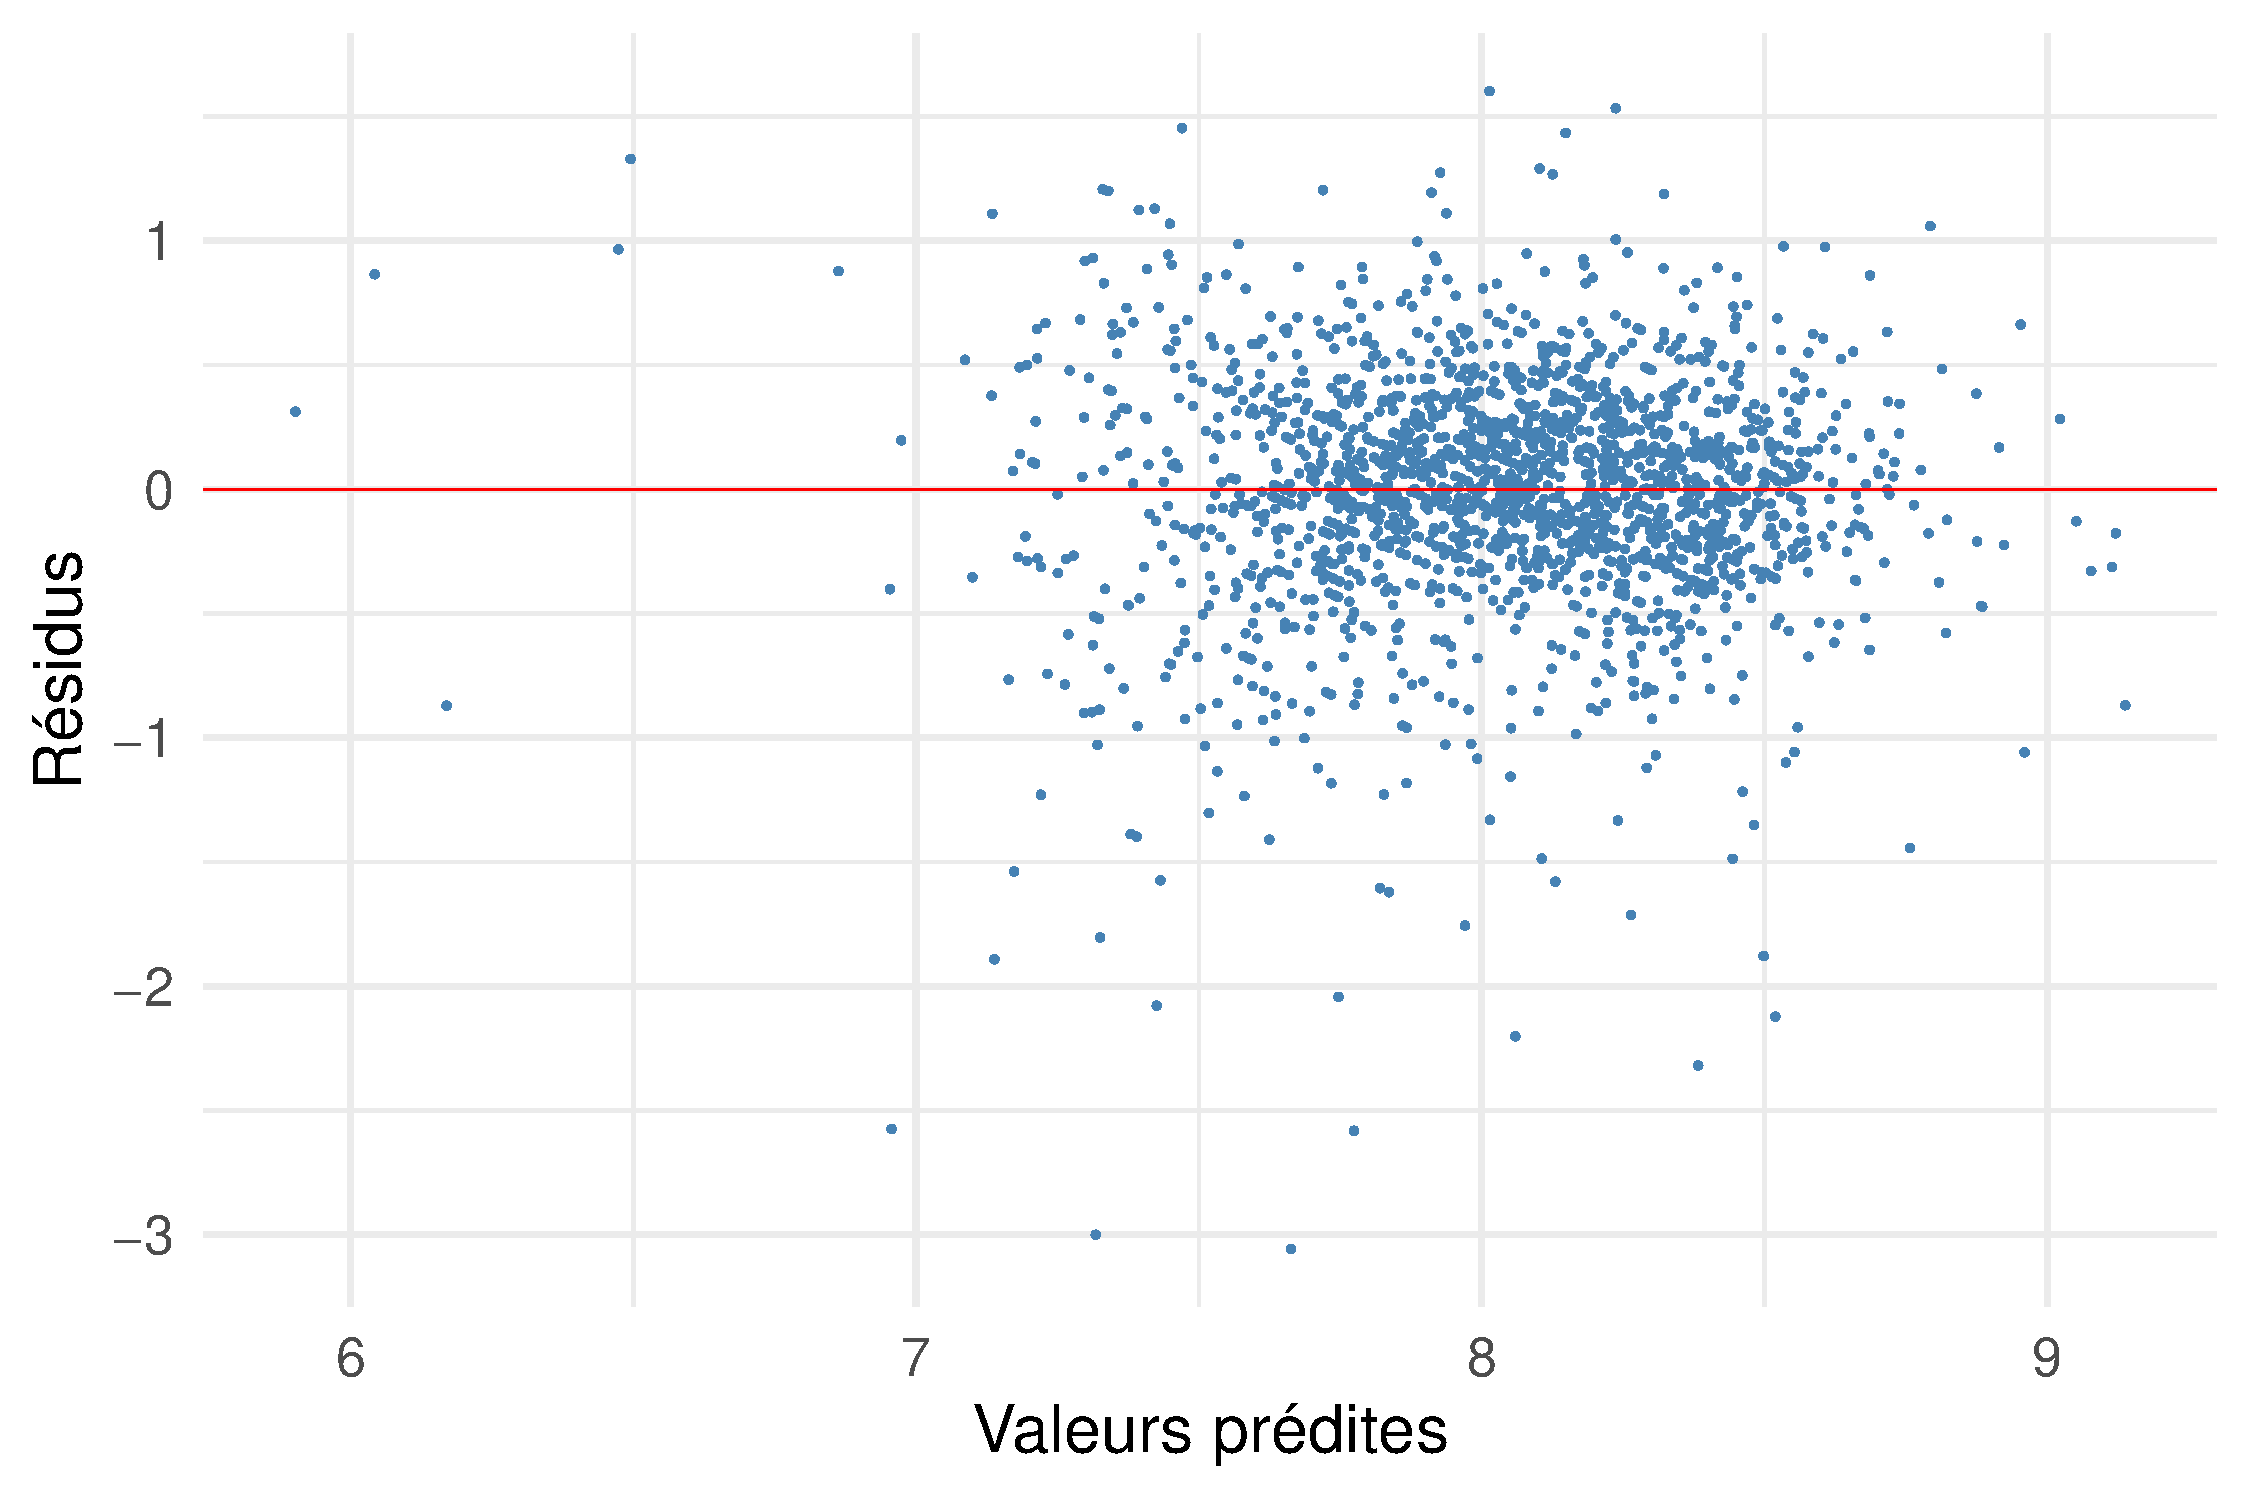
\includegraphics[width=0.49\linewidth]{figure/plot_hetero_fitted.pdf}
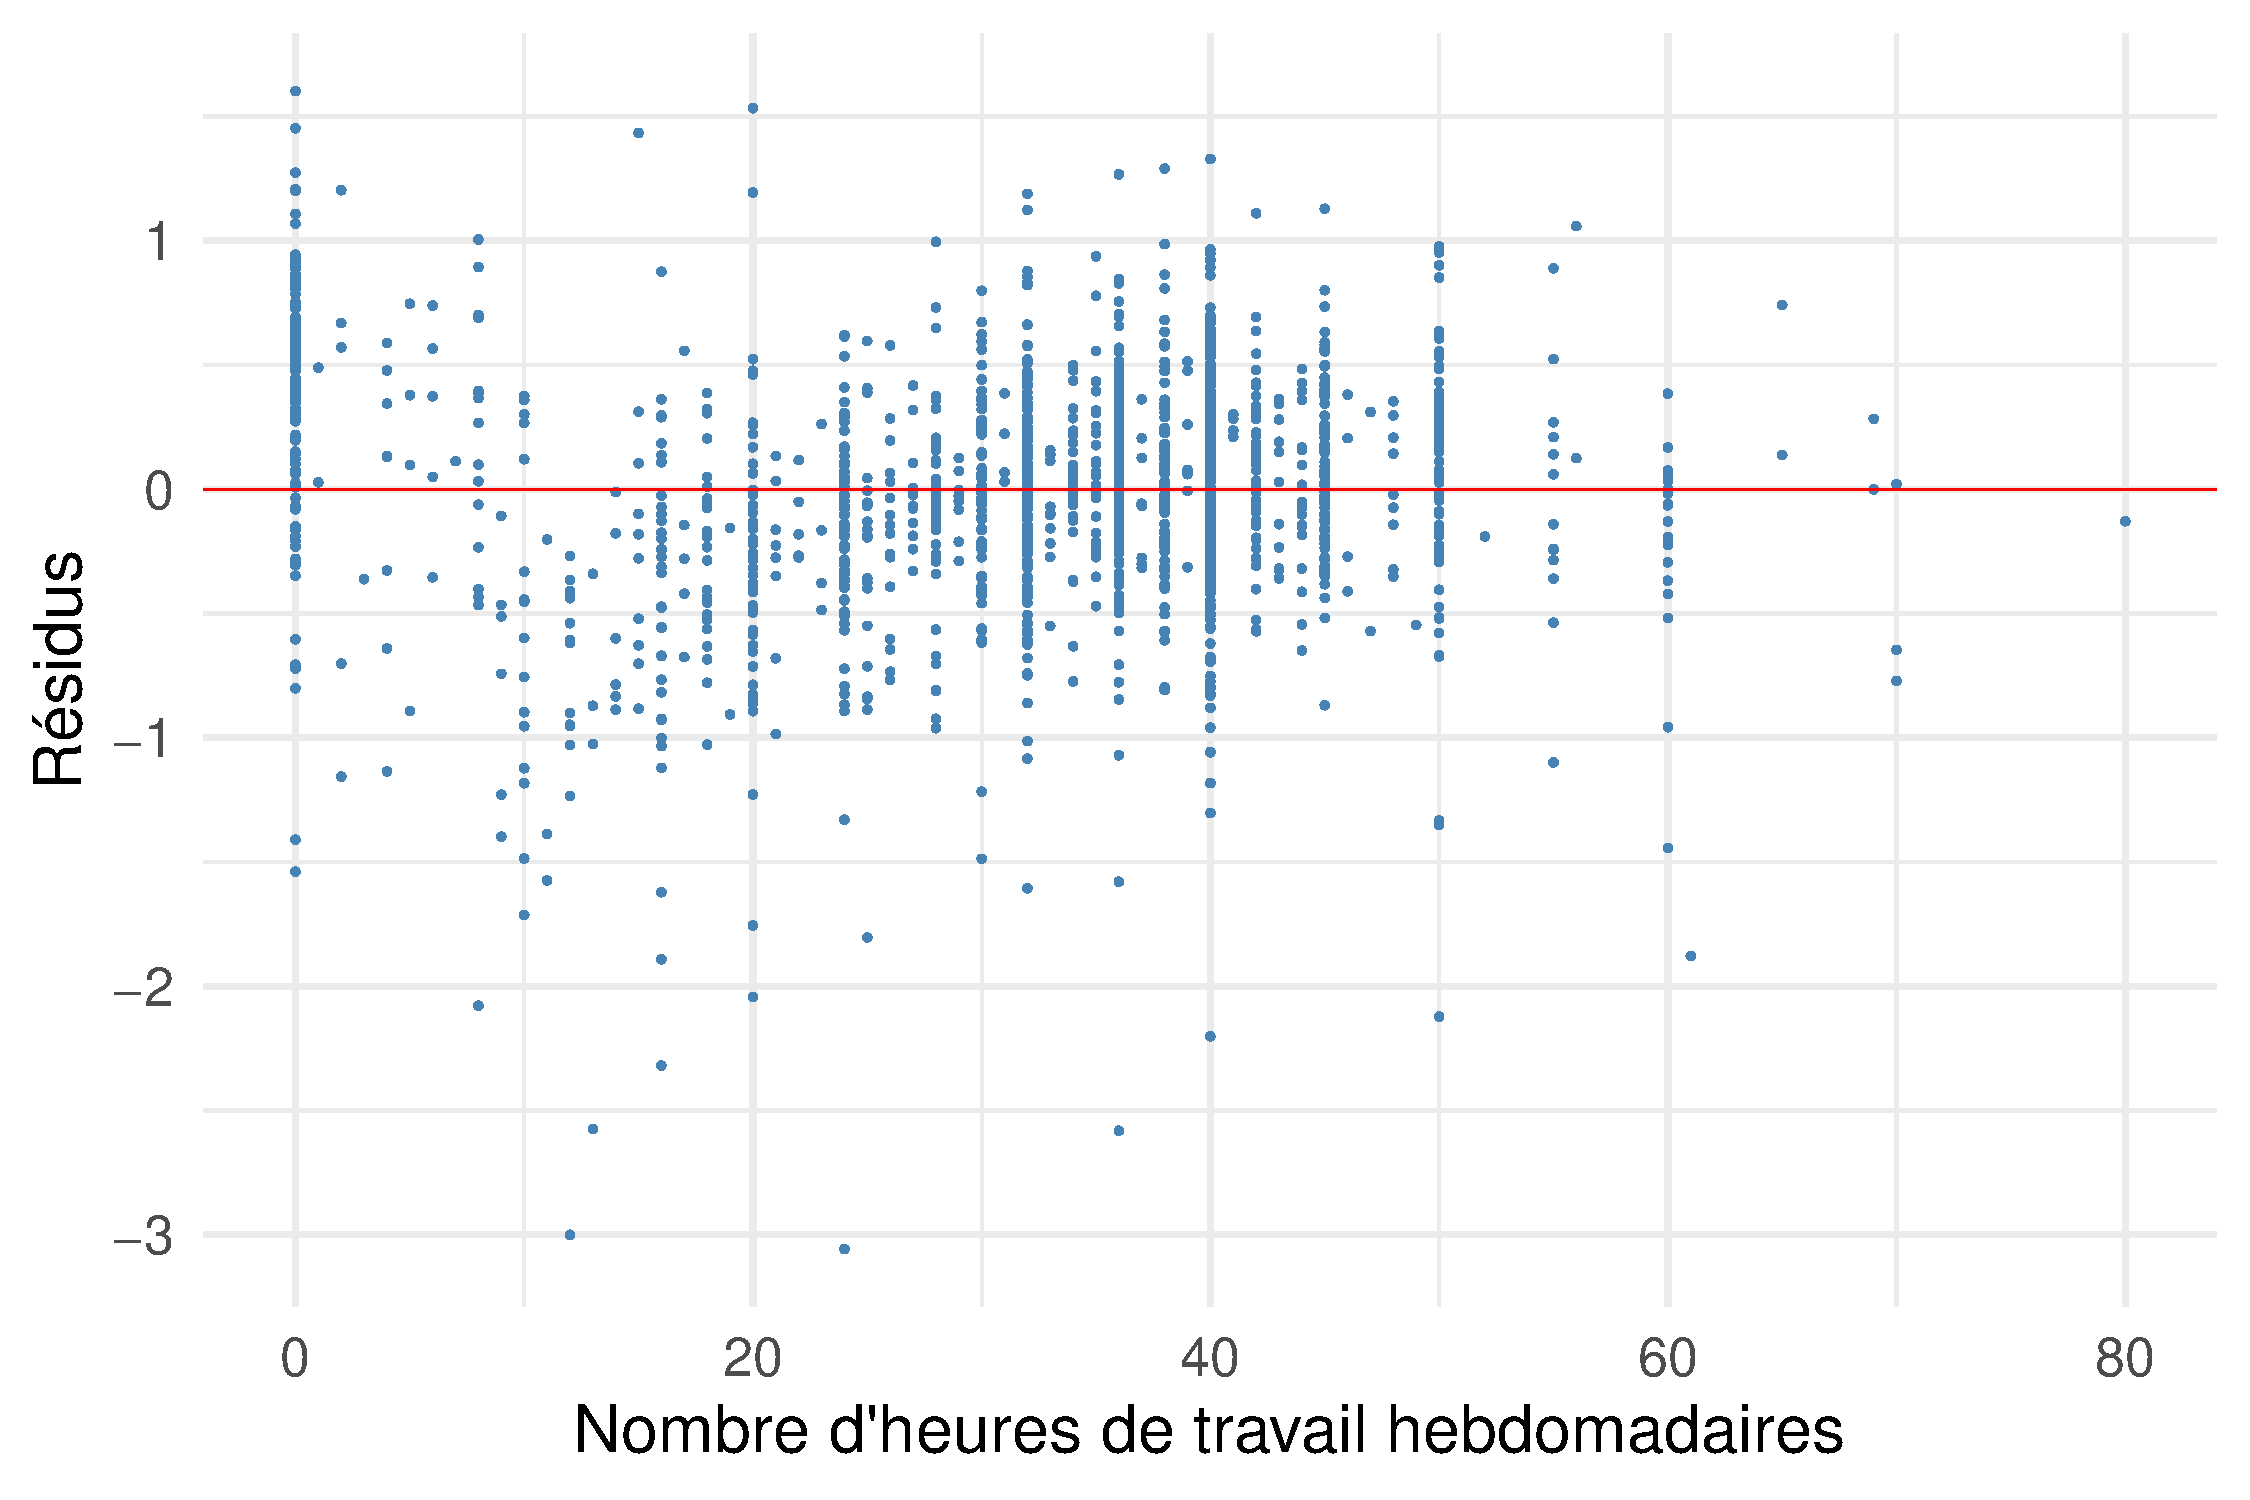
\includegraphics[width=0.49\linewidth]{figure/plot_hetero_heures.pdf}
\caption{Répartition des résidus en fonction des valeurs prédites et de la variable heures\label{fig:hetero}}
\end{figure}

\subsection{Détection de l’endogénéité et pistes de correction}

\section{Résultats principaux}

\section{Analyse et mise en perspective des résultats}

Et ici on peut écrire ... et insérer des blocs de code qui s'éxécutent, avec le code et le résultat qui s'affichent

\begin{knitrout}
\definecolor{shadecolor}{rgb}{0.969, 0.969, 0.969}\color{fgcolor}\begin{kframe}
\begin{alltt}
\hlstd{a} \hlkwb{<-}  \hlnum{2}\hlopt{+}\hlnum{2}
\hlstd{a}
\end{alltt}
\begin{verbatim}
## [1] 4
\end{verbatim}
\end{kframe}
\end{knitrout}

ou juste le résultat : 

\begin{knitrout}
\definecolor{shadecolor}{rgb}{0.969, 0.969, 0.969}\color{fgcolor}\begin{kframe}
\begin{verbatim}
## [1] 6
\end{verbatim}
\end{kframe}
\end{knitrout}

ou totalement invisibles : 


Et ensuite on peut citer les résultats : à première vue $4 < 6$ mais je crois que c'est 8 qui est le plus grand.




\begin{figure}[h]
\center
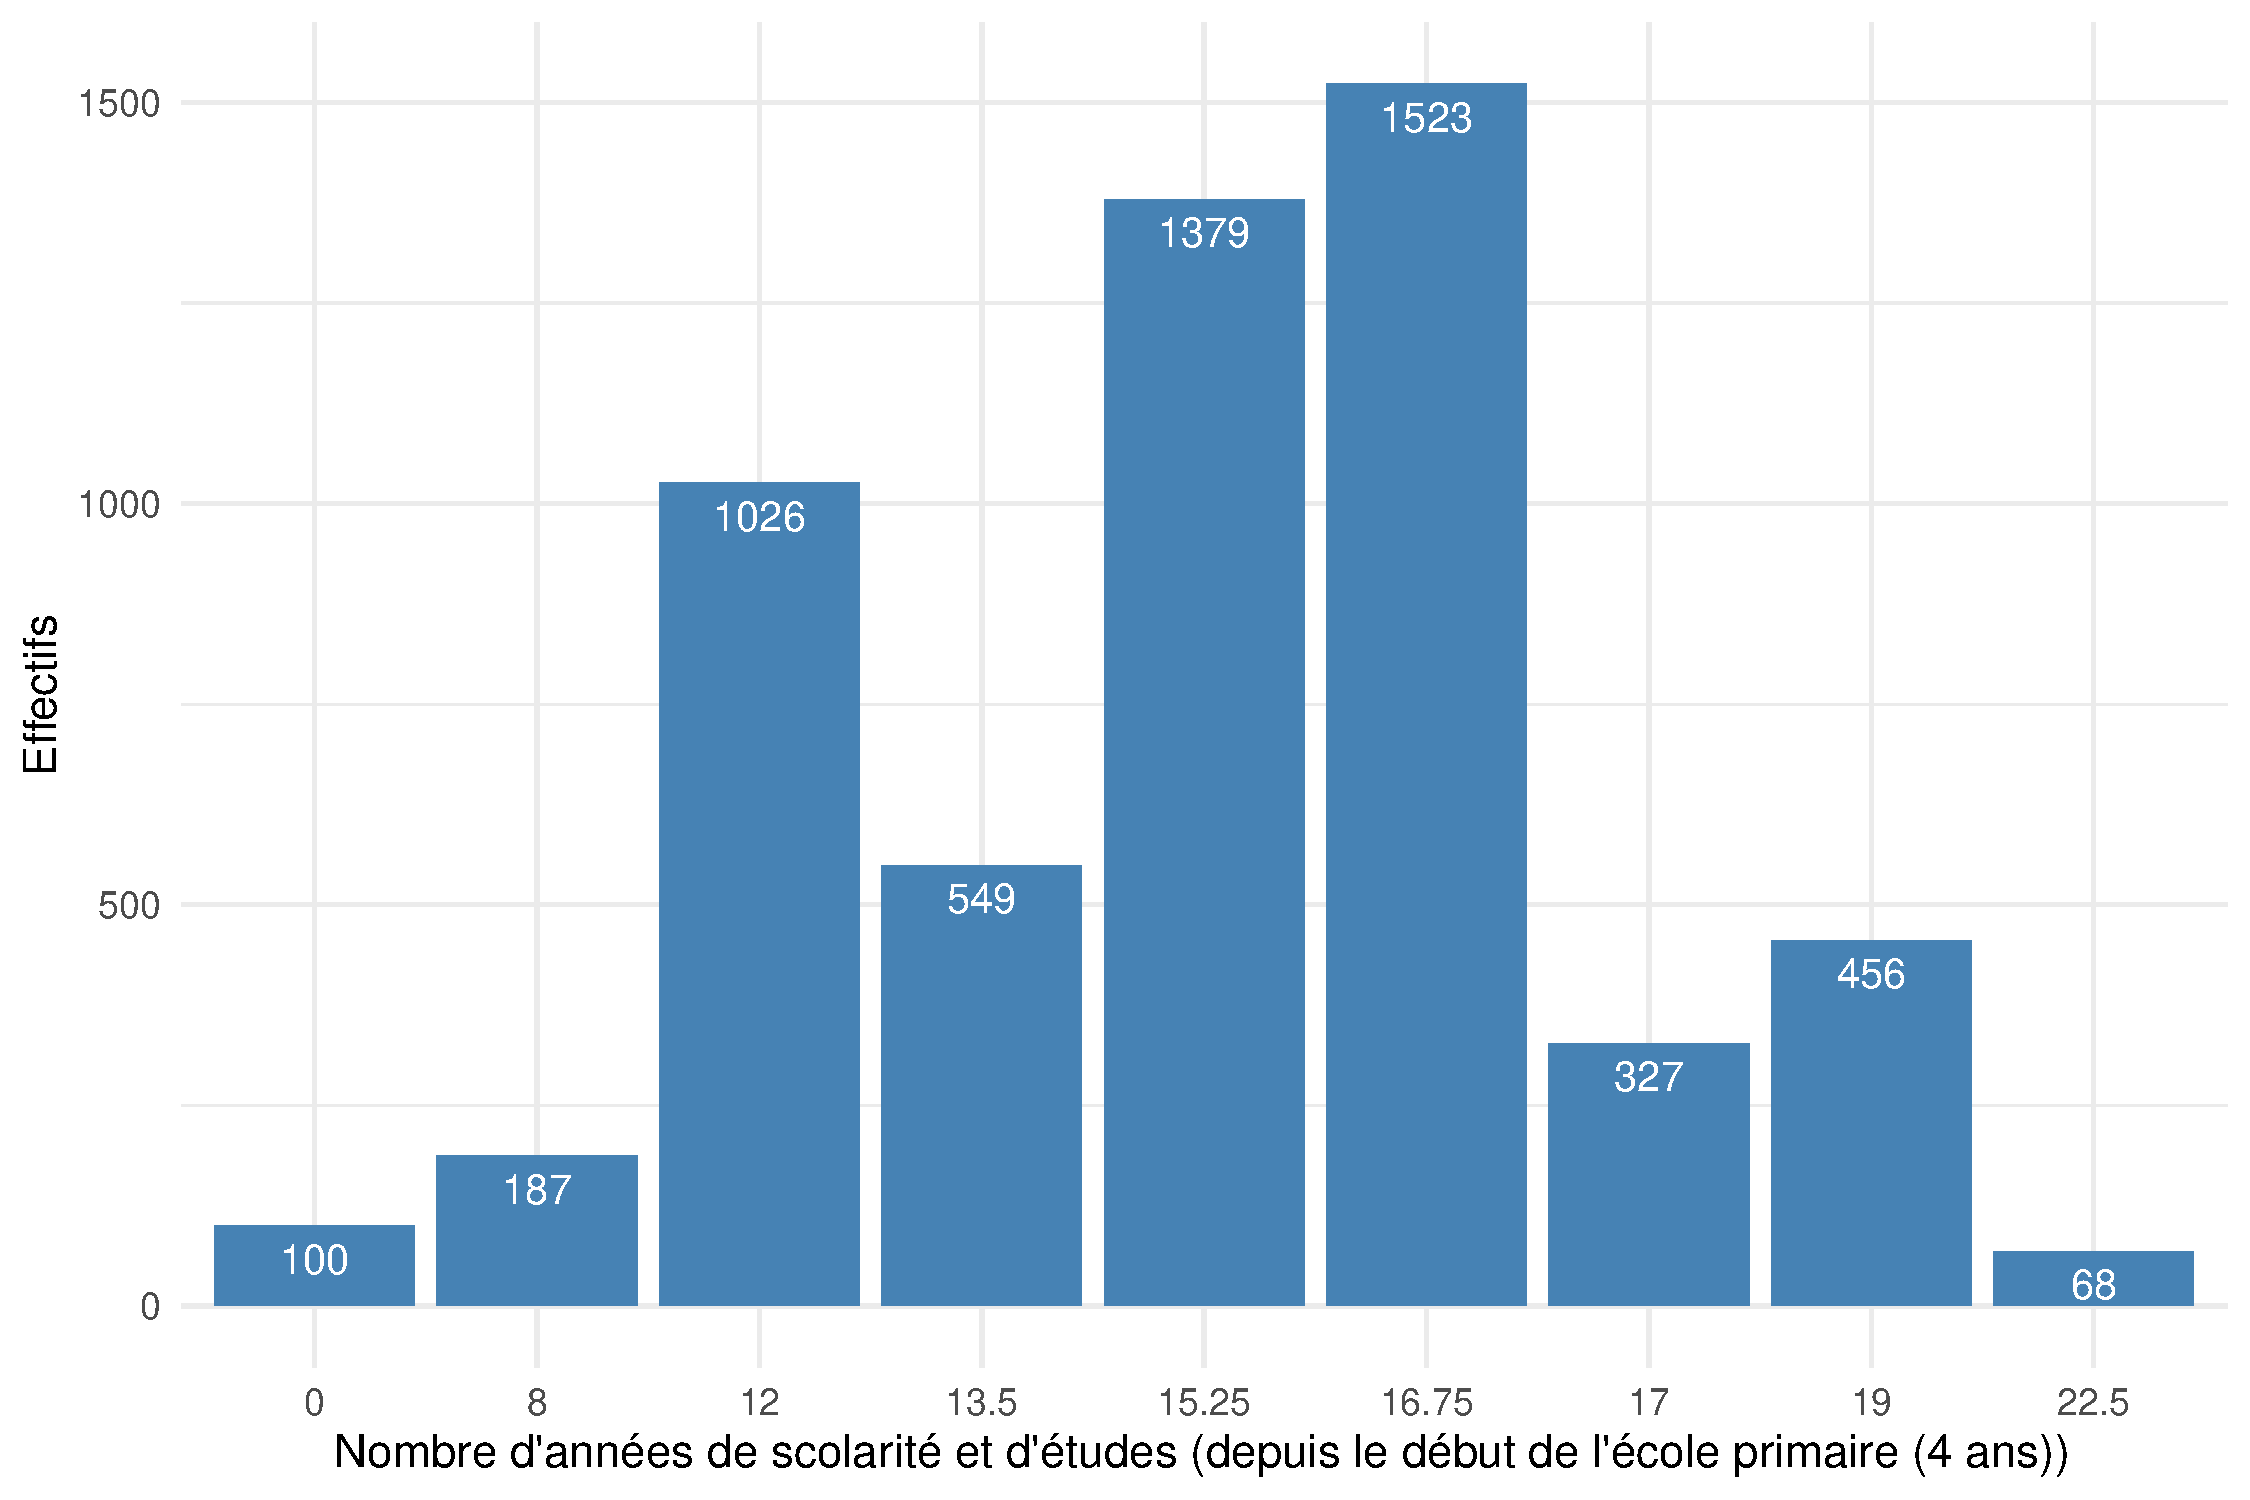
\includegraphics[width=0.7\linewidth]{figure/educ.pdf}
\caption{Niveau d'éducation (avec diplôme) des individus de l'échantillon}
\end{figure}

\begin{knitrout}
\definecolor{shadecolor}{rgb}{0.969, 0.969, 0.969}\color{fgcolor}\begin{kframe}
\begin{verbatim}
## [1] 5615
## [1] 0
\end{verbatim}
\end{kframe}
\end{knitrout}

% latex table generated in R 4.2.1 by xtable 1.8-4 package
% Mon May 15 04:20:17 2023
\begin{table}[ht]
\centering
\caption{Tableau des résidus} 
\label{tb:lm1}
\begin{tabular}{rrrrr}
  \toprule
 & Estimate & Std. Error & t value & Pr($>$$|$t$|$) \\ 
  \midrule
(Intercept) & 5.8617 & 0.0959 & 61.13 & 0.0000 \\ 
  data\$age & 0.0078 & 0.0010 & 7.77 & 0.0000 \\ 
  data\$genre & -0.3036 & 0.0222 & -13.70 & 0.0000 \\ 
  data\$heures & 0.0140 & 0.0008 & 17.01 & 0.0000 \\ 
  data\$experience & 0.0030 & 0.0011 & 2.65 & 0.0081 \\ 
  data\$nbenfants & -0.0072 & 0.0095 & -0.76 & 0.4483 \\ 
  data\$education & 0.0922 & 0.0046 & 19.93 & 0.0000 \\ 
   \bottomrule
\end{tabular}
\end{table}


\printbibliography
\end{document}
